\documentclass[a4paper]{ctexart}
\usepackage{xeCJK}
\usepackage{setspace}
\usepackage{graphicx,wrapfig}
\usepackage{fontspec,xunicode,xltxtra}
\usepackage{fancyhdr,titlesec,titletoc}
\usepackage[titletoc]{appendix}
\usepackage[top=29mm,bottom=29mm,left=31.8mm,right=31.8mm]{geometry}
\usepackage{enumerate,enumitem}
\usepackage{caption}
\usepackage{amsmath,amssymb,bm,array}
\usepackage{cite}
\usepackage{diagbox}
\usepackage{algorithm,algorithmicx,algpseudocode}
\usepackage{multirow}
\usepackage[super]{gbt7714}
\setmainfont{Times New Roman}
\setCJKmainfont[BoldFont={Songti SC Bold}]{SimSun}
\setCJKfamilyfont{heiti}{SimHei}
\renewcommand{\heiti}{\CJKfamily{heiti}\fontspec{Times New Roman}}

\newcommand{\mycaptionfont}{\heiti\zihao{5}}
\captionsetup[figure]{name={\mycaptionfont 图},labelsep=period}
\captionsetup[table]{name={\mycaptionfont 表},labelsep=period}
\floatname{algorithm}{\mycaptionfont 算法}
\captionsetup[algorithm]{labelsep=period}
\renewcommand{\captionfont}{\mycaptionfont}
\renewcommand{\captionlabelfont}{\mycaptionfont}

\ctexset {
	section = {
		number = \arabic{section},
		format = \zihao{4}\bfseries,
	},
	subsection = {
		number = \arabic{section}.\arabic{subsection},
		format = \zihao{-4}\bfseries,
	},
	subsubsection = {
		number = \arabic{section}.\arabic{subsection}.\arabic{subsubsection},
		format = \zihao{-4}\bfseries,
	}
}
\setlist[enumerate]{itemindent=2em,listparindent=2em,leftmargin=0em,label=\arabic*、}

\setlength\parskip{.5\baselineskip}
\fancypagestyle{plain}{\pagestyle{fancy}}%改变章节首页页眉
\pagestyle{fancy}
\lhead{}
\chead{视觉物联网技术实验报告}
\rhead{}
\cfoot{\thepage}

\begin{document}
\begin{titlepage}
	\begin{center}
		
\includegraphics[width=0.9\textwidth]{figure//Njust.png}\\
		\vspace{10mm}
		\textbf{\zihao{2}\kaishu{物联网工程学院}}\\[0.8cm]
		\textbf{\zihao{2}\kaishu{视觉物联网技术实验报告}}\\[3cm]
		\textbf{\zihao{2}\kaishu{实验三~动态视觉标签定位(运动目标分割) }}\\[3cm]
		\vspace{\fill}
		\setlength{\extrarowheight}{3mm}
		{\songti\zihao{3}
			\begin{tabular}{rl}
				{\makebox[4\ccwd][s]{班\qquad 级:}} & ~\kaishu 物联1601   \\
				{\makebox[4\ccwd][s]{姓\qquad 名:}} & ~\kaishu 尹达恒     \\
				{\makebox[4\ccwd][s]{学\qquad 号:}} & ~\kaishu 1030616134 \\
				{\makebox[4\ccwd][s]{指导老师:}}    & ~\kaishu 陈莹       \\
			\end{tabular}
		}\\[2cm]
		\vspace{\fill}
		\zihao{4}
		2018\textasciitilde 2019第二学期\\
		2019年5月
	\end{center}
\end{titlepage}

\renewcommand{\baselinestretch}{1.3}
\zihao{-4}
\section{实验目的}
\begin{enumerate}[label=\arabic*、]
	\item 采用差分法,背景差法实现运动目标提取,基本掌握运动目标提取的基本原理和方法;
	\item 了解不同帧率、不同运动速度条件下对检测结果的影响。
\end{enumerate}

\section{实验内容}
\begin{enumerate}[label=\arabic*、]
	\item 利用MATLAB读取图像的基本命令imread和读取视频的基本命令aviread或mmreader;
	\item 调用各种运动目标检测函数进行运动目标分割;
	\item 利用MATLAB形态学算子调整分割结果;
	\item 了解形态学滤波中结构元strel命令的调用格式,通过改变结构元形状和大小,比较运动目标检测效果。
\end{enumerate}

\section{实验步骤}
\subsection{图像分割}\label{sec:图像分割}
\subsubsection{使用帧差法进行动态图像分割}
由于实验指导中给出的Matlab代码无法运行,本实验按照帧差法的程序逻辑采用Python和Opencv自行编写帧差法程序。实验步骤如下:
\begin{enumerate}[label=\arabic*、]
	\item 编写帧差法程序“帧差.py”,选择运动判定阈值为100,帧差数为1;
	\item 运行程序得到结果“帧差1.avi”;
	\item 调整“帧差.py”程序中的帧差数得到一系列不同的帧差结果“帧差XX.avi”;
	\item 从每个实验结果中的运动幅度较大的部分分别选出一帧进行分割效果对比,结果如图\ref{figure:帧差法}。
\end{enumerate}
\begin{figure}[htbp]
	\centering
	\begin{minipage}[t]{0.2\textwidth}
		\centering
		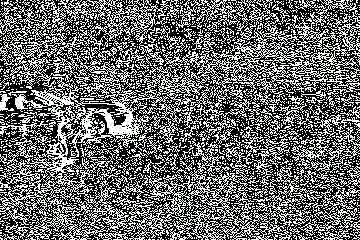
\includegraphics[width=\textwidth]{figure/frames/sb1400.jpg}
	\end{minipage}
	\begin{minipage}[t]{0.2\textwidth}
		\centering
		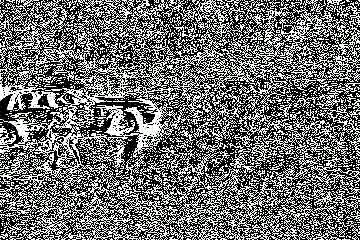
\includegraphics[width=\textwidth]{figure/frames/sb1405.jpg}
	\end{minipage}
	\begin{minipage}[t]{0.2\textwidth}
		\centering
		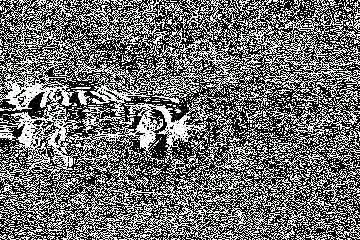
\includegraphics[width=\textwidth]{figure/frames/sb1410.jpg}
	\end{minipage}
	\begin{minipage}[t]{0.2\textwidth}
		\centering
		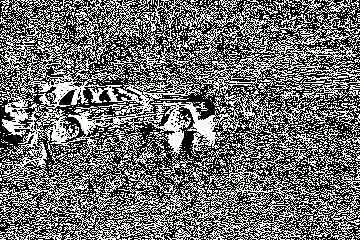
\includegraphics[width=\textwidth]{figure/frames/sb1415.jpg}
	\end{minipage}\\
	\begin{minipage}[t]{0.2\textwidth}
		\centering
		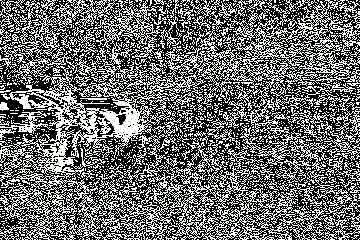
\includegraphics[width=\textwidth]{figure/frames/sb2400.jpg}
	\end{minipage}
	\begin{minipage}[t]{0.2\textwidth}
		\centering
		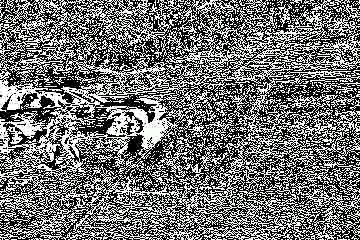
\includegraphics[width=\textwidth]{figure/frames/sb2405.jpg}
	\end{minipage}
	\begin{minipage}[t]{0.2\textwidth}
		\centering
		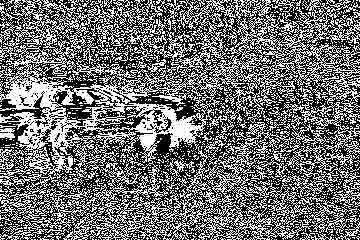
\includegraphics[width=\textwidth]{figure/frames/sb2410.jpg}
	\end{minipage}
	\begin{minipage}[t]{0.2\textwidth}
		\centering
		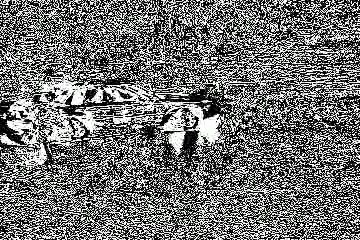
\includegraphics[width=\textwidth]{figure/frames/sb2415.jpg}
	\end{minipage}\\
	\begin{minipage}[t]{0.2\textwidth}
		\centering
		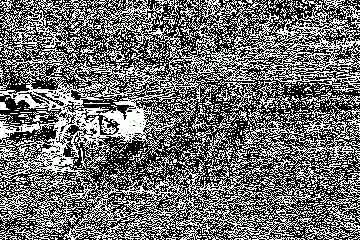
\includegraphics[width=\textwidth]{figure/frames/sb3400.jpg}
	\end{minipage}
	\begin{minipage}[t]{0.2\textwidth}
		\centering
		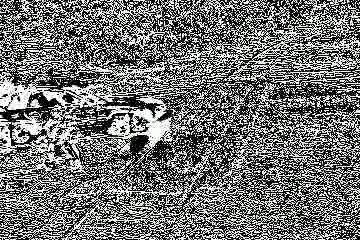
\includegraphics[width=\textwidth]{figure/frames/sb3405.jpg}
	\end{minipage}
	\begin{minipage}[t]{0.2\textwidth}
		\centering
		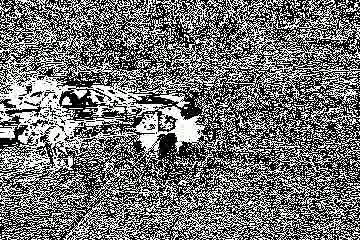
\includegraphics[width=\textwidth]{figure/frames/sb3410.jpg}
	\end{minipage}
	\begin{minipage}[t]{0.2\textwidth}
		\centering
		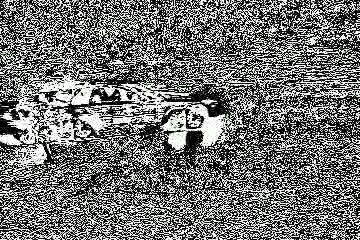
\includegraphics[width=\textwidth]{figure/frames/sb3415.jpg}
	\end{minipage}\\
	\begin{minipage}[t]{0.2\textwidth}
		\centering
		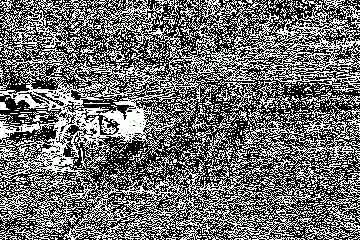
\includegraphics[width=\textwidth]{figure/frames/sb3400.jpg}
	\end{minipage}
	\begin{minipage}[t]{0.2\textwidth}
		\centering
		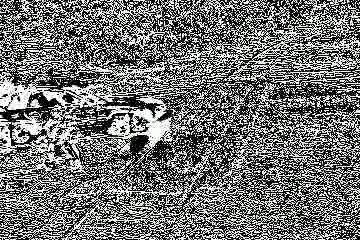
\includegraphics[width=\textwidth]{figure/frames/sb3405.jpg}
	\end{minipage}
	\begin{minipage}[t]{0.2\textwidth}
		\centering
		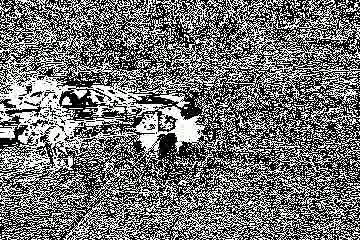
\includegraphics[width=\textwidth]{figure/frames/sb3410.jpg}
	\end{minipage}
	\begin{minipage}[t]{0.2\textwidth}
		\centering
		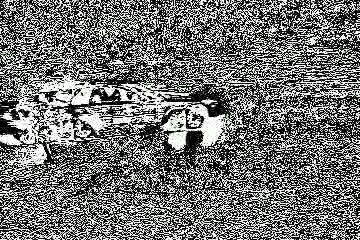
\includegraphics[width=\textwidth]{figure/frames/sb3415.jpg}
	\end{minipage}
	\caption{帧差法(从上到下帧差间隔分别为1帧、2帧、3帧、4帧)}\label{figure:帧差法}
\end{figure}
\subsubsection{使用时间平均法进行动态图像分割}
由于实验指导中给出的Matlab代码无法运行,本实验按照时间平均法的程序逻辑采用Python和Opencv自行编写时间平均法程序。实验步骤如下:
\begin{enumerate}[label=\arabic*、]
	\item 编写时间平均法程序“时间平均.py”,选择运动判定阈值为100,计算平均值所用的帧数为9;
	\item 运行程序得到结果“时间平均9.avi”;
	\item 调整“时间平均.py”程序中计算平均值所用的帧数得到一系列不同的时间平均结果“时间平均XX.avi”;
	\item 从每个实验结果中的运动幅度较大的部分分别选出一帧进行分割效果对比,结果如图\ref{figure:时间平均法}。
	\begin{figure}[htbp]
		\centering
		\begin{minipage}[t]{0.2\textwidth}
			\centering
			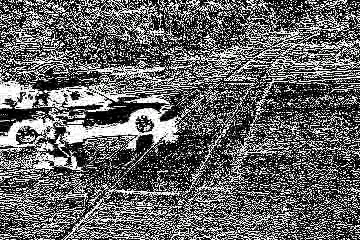
\includegraphics[width=\textwidth]{figure/frames/avg9400.jpg}
		\end{minipage}
		\begin{minipage}[t]{0.2\textwidth}
			\centering
			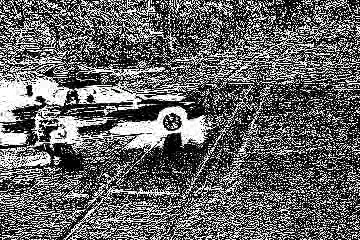
\includegraphics[width=\textwidth]{figure/frames/avg9405.jpg}
		\end{minipage}
		\begin{minipage}[t]{0.2\textwidth}
			\centering
			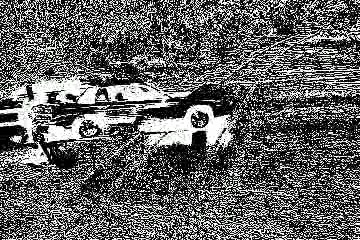
\includegraphics[width=\textwidth]{figure/frames/avg9410.jpg}
		\end{minipage}
		\begin{minipage}[t]{0.2\textwidth}
			\centering
			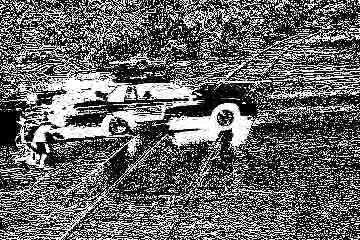
\includegraphics[width=\textwidth]{figure/frames/avg9415.jpg}
		\end{minipage}\\
		\begin{minipage}[t]{0.2\textwidth}
			\centering
			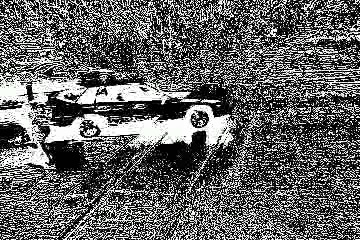
\includegraphics[width=\textwidth]{figure/frames/avg19400.jpg}
		\end{minipage}
		\begin{minipage}[t]{0.2\textwidth}
			\centering
			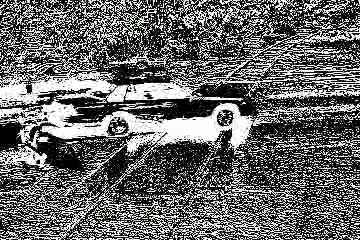
\includegraphics[width=\textwidth]{figure/frames/avg19405.jpg}
		\end{minipage}
		\begin{minipage}[t]{0.2\textwidth}
			\centering
			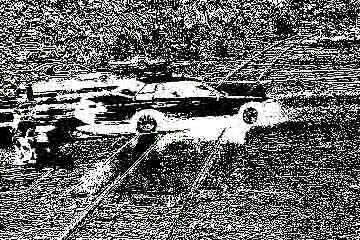
\includegraphics[width=\textwidth]{figure/frames/avg19410.jpg}
		\end{minipage}
		\begin{minipage}[t]{0.2\textwidth}
			\centering
			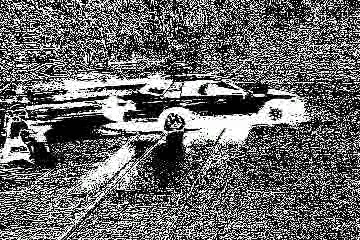
\includegraphics[width=\textwidth]{figure/frames/avg19415.jpg}
		\end{minipage}\\
		\begin{minipage}[t]{0.2\textwidth}
			\centering
			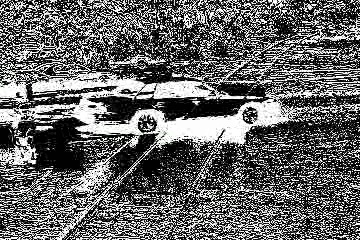
\includegraphics[width=\textwidth]{figure/frames/avg29400.jpg}
		\end{minipage}
		\begin{minipage}[t]{0.2\textwidth}
			\centering
			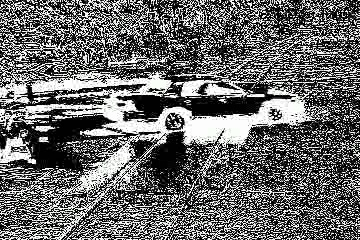
\includegraphics[width=\textwidth]{figure/frames/avg29405.jpg}
		\end{minipage}
		\begin{minipage}[t]{0.2\textwidth}
			\centering
			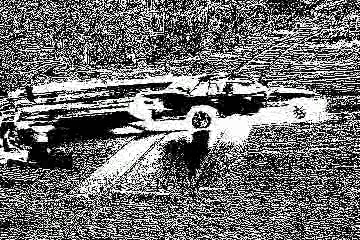
\includegraphics[width=\textwidth]{figure/frames/avg29410.jpg}
		\end{minipage}
		\begin{minipage}[t]{0.2\textwidth}
			\centering
			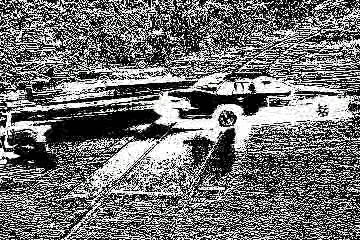
\includegraphics[width=\textwidth]{figure/frames/avg29415.jpg}
		\end{minipage}\\
		\begin{minipage}[t]{0.2\textwidth}
			\centering
			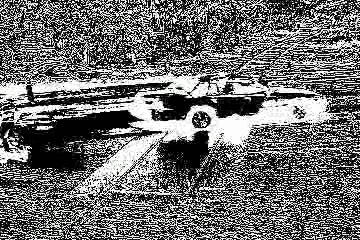
\includegraphics[width=\textwidth]{figure/frames/avg39400.jpg}
		\end{minipage}
		\begin{minipage}[t]{0.2\textwidth}
			\centering
			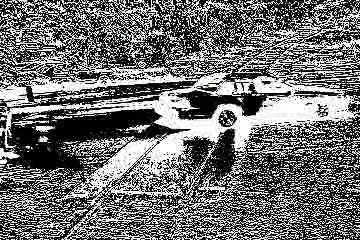
\includegraphics[width=\textwidth]{figure/frames/avg39405.jpg}
		\end{minipage}
		\begin{minipage}[t]{0.2\textwidth}
			\centering
			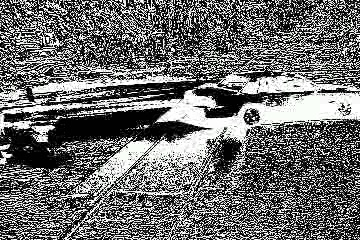
\includegraphics[width=\textwidth]{figure/frames/avg39410.jpg}
		\end{minipage}
		\begin{minipage}[t]{0.2\textwidth}
			\centering
			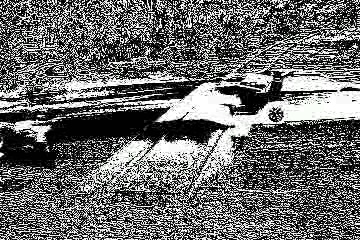
\includegraphics[width=\textwidth]{figure/frames/avg39415.jpg}
		\end{minipage}\\
		\begin{minipage}[t]{0.2\textwidth}
			\centering
			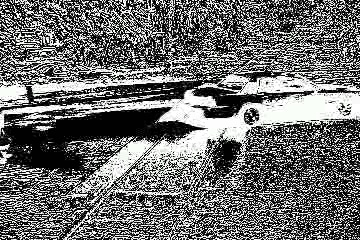
\includegraphics[width=\textwidth]{figure/frames/avg49400.jpg}
		\end{minipage}
		\begin{minipage}[t]{0.2\textwidth}
			\centering
			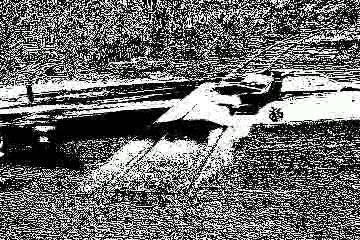
\includegraphics[width=\textwidth]{figure/frames/avg49405.jpg}
		\end{minipage}
		\begin{minipage}[t]{0.2\textwidth}
			\centering
			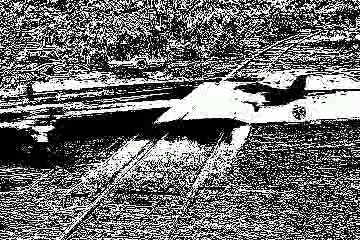
\includegraphics[width=\textwidth]{figure/frames/avg49410.jpg}
		\end{minipage}
		\begin{minipage}[t]{0.2\textwidth}
			\centering
			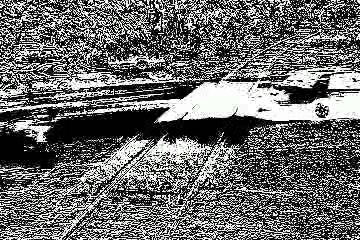
\includegraphics[width=\textwidth]{figure/frames/avg49415.jpg}
		\end{minipage}\\
		\caption{背景差法(从上到下分别为9帧取平均、19帧取平均、29帧取平均、39帧取平均、49帧取平均)}\label{figure:时间平均法}
	\end{figure}
\end{enumerate}
\subsubsection{使用单高斯法进行动态图像分割}
实验指导中给出的单高斯法程序Matlab代码在修改视频读取方法后可以在Matlab R2015b平台运行。实验步骤如下:
\begin{enumerate}[label=\arabic*、]
	\item 修改实验指导中给出的单高斯法程序,将其中的视频读取方法修改为VideoReader方法,保持程序中的训练帧和阈值两个参数不变,形成程序文件\newline“single\_gaussians.m”;
	\item 运行程序得到结果“单高斯.avi”;
	\item 调整“single\_gaussians.m”程序中的训练帧和阈值两个参数得到一系列不同的单高斯结果“单高斯X.avi”;
	\item 从每个实验结果中的运动幅度较大的部分分别选出一帧进行分割效果对比,结果如图\ref{figure:单高斯法}。
\end{enumerate}
\begin{figure}[htbp]
	\centering
	\begin{minipage}[t]{0.2\textwidth}
		\centering
		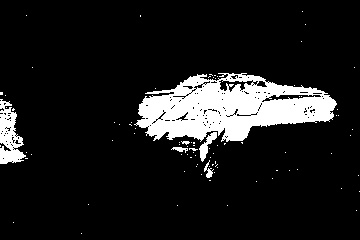
\includegraphics[width=\textwidth]{figure/frames/single_gT01400.jpg}
	\end{minipage}
	\begin{minipage}[t]{0.2\textwidth}
		\centering
		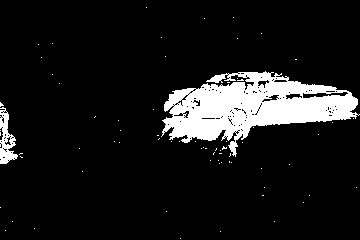
\includegraphics[width=\textwidth]{figure/frames/single_gT01405.jpg}
	\end{minipage}
	\begin{minipage}[t]{0.2\textwidth}
		\centering
		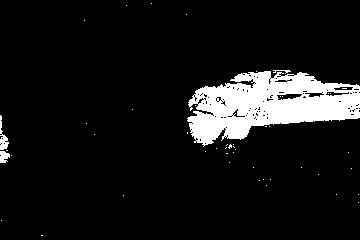
\includegraphics[width=\textwidth]{figure/frames/single_gT01410.jpg}
	\end{minipage}
	\begin{minipage}[t]{0.2\textwidth}
		\centering
		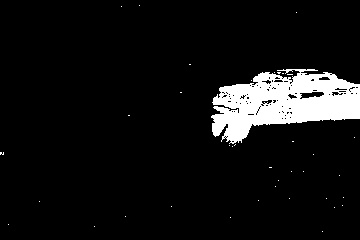
\includegraphics[width=\textwidth]{figure/frames/single_gT01415.jpg}
	\end{minipage}\\
	\begin{minipage}[t]{0.2\textwidth}
		\centering
		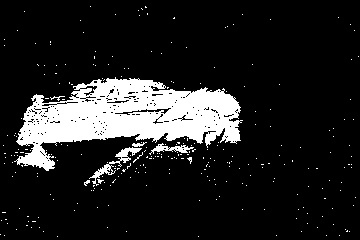
\includegraphics[width=\textwidth]{figure/frames/single_gN20400.jpg}
	\end{minipage}
	\begin{minipage}[t]{0.2\textwidth}
		\centering
		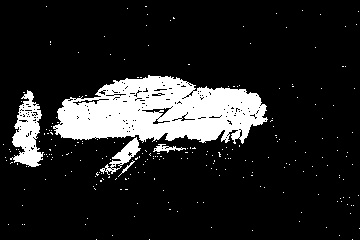
\includegraphics[width=\textwidth]{figure/frames/single_gN20405.jpg}
	\end{minipage}
	\begin{minipage}[t]{0.2\textwidth}
		\centering
		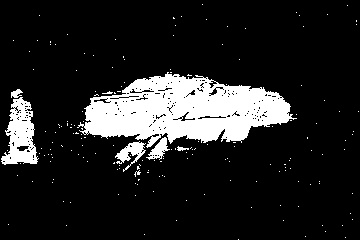
\includegraphics[width=\textwidth]{figure/frames/single_gN20410.jpg}
	\end{minipage}
	\begin{minipage}[t]{0.2\textwidth}
		\centering
		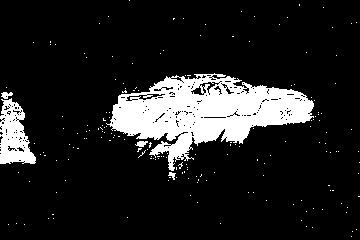
\includegraphics[width=\textwidth]{figure/frames/single_gN20415.jpg}
	\end{minipage}\\
	\begin{minipage}[t]{0.2\textwidth}
		\centering
		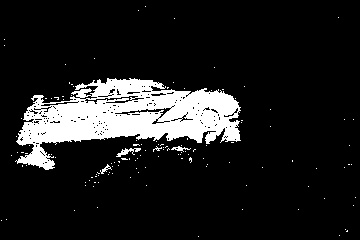
\includegraphics[width=\textwidth]{figure/frames/single_gN20T01400.jpg}
	\end{minipage}
	\begin{minipage}[t]{0.2\textwidth}
		\centering
		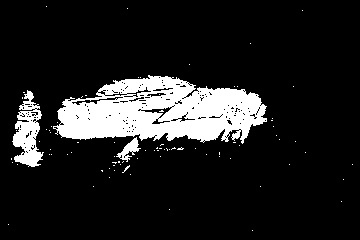
\includegraphics[width=\textwidth]{figure/frames/single_gN20T01405.jpg}
	\end{minipage}
	\begin{minipage}[t]{0.2\textwidth}
		\centering
		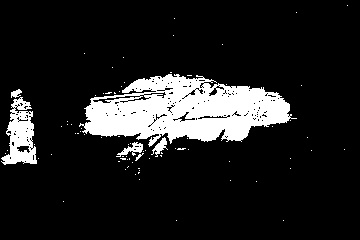
\includegraphics[width=\textwidth]{figure/frames/single_gN20T01410.jpg}
	\end{minipage}
	\begin{minipage}[t]{0.2\textwidth}
		\centering
		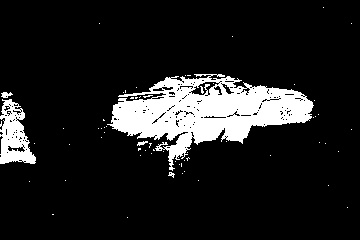
\includegraphics[width=\textwidth]{figure/frames/single_gN20T01415.jpg}
	\end{minipage}\\
	\begin{minipage}[t]{0.2\textwidth}
		\centering
		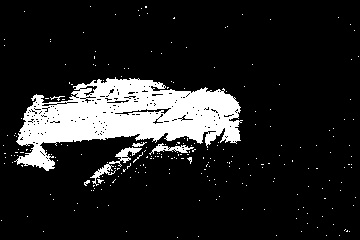
\includegraphics[width=\textwidth]{figure/frames/single_gN80340.jpg}
	\end{minipage}
	\begin{minipage}[t]{0.2\textwidth}
		\centering
		\includegraphics[width=\textwidth]{figure/frames/single_gN80345.jpg}
	\end{minipage}
	\begin{minipage}[t]{0.2\textwidth}
		\centering
		\includegraphics[width=\textwidth]{figure/frames/single_gN80350.jpg}
	\end{minipage}
	\begin{minipage}[t]{0.2\textwidth}
		\centering
		\includegraphics[width=\textwidth]{figure/frames/single_gN80355.jpg}
	\end{minipage}
	\caption{单高斯法(从上到下分别为阈值减小为$1\times10^{-4}$、训练帧数减小为20、阈值减小为$1\times10^{-4}$且训练帧数减小为20、训练帧数增大为80)}\label{figure:单高斯法}
\end{figure}
\subsubsection{使用混合高斯法进行动态图像分割}
实验指导中给出的MOG混合高斯法Matlab代码在修改视频读取方法后可以在Matlab R2015b平台运行。实验步骤如下:
\begin{enumerate}[label=\arabic*、]
	\item 编写混合高斯法程序“mixture\_gaussians.m”得到结果“混合高斯001.avi”;调整“mixture\_gaussians.m”程序中的混合高斯法的阈值参数得到一系列不同的混合高斯结果“混合高斯XXX.avi”;
	\item 从每个实验结果中的运动幅度较大的部分分别选出一帧进行分割效果对比,结果如图\ref{figure:混合高斯法}。
\end{enumerate}
\begin{figure}[htbp]
	\centering
	\begin{minipage}[t]{0.2\textwidth}
		\centering
		\includegraphics[width=\textwidth]{figure/frames/mixture_of_gaussians_output400.jpg}
	\end{minipage}
	\begin{minipage}[t]{0.2\textwidth}
		\centering
		\includegraphics[width=\textwidth]{figure/frames/mixture_of_gaussians_output405.jpg}
	\end{minipage}
	\begin{minipage}[t]{0.2\textwidth}
		\centering
		\includegraphics[width=\textwidth]{figure/frames/mixture_of_gaussians_output410.jpg}
	\end{minipage}
	\begin{minipage}[t]{0.2\textwidth}
		\centering
		\includegraphics[width=\textwidth]{figure/frames/mixture_of_gaussians_output415.jpg}
	\end{minipage}
	\caption{混合高斯法}\label{figure:混合高斯法}
\end{figure}

\section{实验结果分析}
\begin{itemize}
	\item 由图\ref{figure:帧差法}可以看出,增加帧差间隔对帧差法的处理效果影响不大,反而会造成鬼影现象,这是由于拍摄视频时摄像机有抖动,造成不同帧背景位置不一样所致;
	\item 由图\ref{figure:时间平均法}可以看出,增加背景平均帧数量对时间平均法的处理效果影响不大,反而会造成更长的拖影。这也是由于拍摄视频时摄像机有抖动,造成不同帧背景位置不一样所致;
	\item 由图\ref{figure:单高斯法}可以看出,减小阈值可以在一定程度上减少单高斯法的结果噪声,但增大训练帧数量对单高斯法的结果影响不大;
	\item 由图\ref{figure:帧差法}、图\ref{figure:时间平均法}、、图\ref{figure:单高斯法}和图\ref{figure:混合高斯法}可以综合看出,基于高斯模型和高斯混合模型的方法在运动目标分割方面具有更好的效果,且能较好的克服背景抖动对目标分割的影响。
\end{itemize}




\end{document}